
\documentclass[conference]{IEEEtran}

\usepackage[pdftex]{graphicx}
\graphicspath{ {../images/} }
\usepackage{caption}
\usepackage{subcaption}
\usepackage{float}
\usepackage{amsmath}

\usepackage{hyperref}
\hypersetup
{
    colorlinks=true,
    linkcolor=black,   
    urlcolor=blue,
    citecolor=black,
}

\usepackage{pdfpages}
\renewcommand{\familydefault}{\sfdefault}

% *** ALIGNMENT PACKAGES ***
%
%\usepackage{array}
% Frank Mittelbach's and David Carlisle's array.sty patches and improves
% the standard LaTeX2e array and tabular environments to provide better
% appearance and additional user controls. As the default LaTeX2e table
% generation code is lacking to the point of almost being broken with
% respect to the quality of the end results, all users are strongly
% advised to use an enhanced (at the very least that provided by array.sty)
% set of table tools. array.sty is already installed on most systems. The
% latest version and documentation can be obtained at:
% http://www.ctan.org/tex-archive/macros/latex/required/tools/


%\usepackage{mdwmath}
%\usepackage{mdwtab}
% Also highly recommended is Mark Wooding's extremely powerful MDW tools,
% especially mdwmath.sty and mdwtab.sty which are used to format equations
% and tables, respectively. The MDWtools set is already installed on most
% LaTeX systems. The lastest version and documentation is available at:
% http://www.ctan.org/tex-archive/macros/latex/contrib/mdwtools/


% IEEEtran contains the IEEEeqnarray family of commands that can be used to
% generate multiline equations as well as matrices, tables, etc., of high
% quality.


% *** SUBFIGURE PACKAGES ***
%\usepackage[tight,footnotesize]{subfigure}
% subfigure.sty was written by Steven Douglas Cochran. This package makes it
% easy to put subfigures in your figures. e.g., "Figure 1a and 1b". For IEEE
% work, it is a good idea to load it with the tight package option to reduce
% the amount of white space around the subfigures. subfigure.sty is already
% installed on most LaTeX systems. The latest version and documentation can
% be obtained at:
% http://www.ctan.org/tex-archive/obsolete/macros/latex/contrib/subfigure/
% subfigure.sty has been superceeded by subfig.sty.


% *** FLOAT PACKAGES ***
%
%\usepackage{fixltx2e}
% fixltx2e, the successor to the earlier fix2col.sty, was written by
% Frank Mittelbach and David Carlisle. This package corrects a few problems
% in the LaTeX2e kernel, the most notable of which is that in current
% LaTeX2e releases, the ordering of single and double column floats is not
% guaranteed to be preserved. Thus, an unpatched LaTeX2e can allow a
% single column figure to be placed prior to an earlier double column
% figure. The latest version and documentation can be found at:
% http://www.ctan.org/tex-archive/macros/latex/base/



\usepackage{stfloats}
% stfloats.sty was written by Sigitas Tolusis. This package gives LaTeX2e
% the ability to do double column floats at the bottom of the page as well
% as the top. (e.g., "\begin{figure*}[!b]" is not normally possible in
% LaTeX2e). It also provides a command:
%\fnbelowfloat
% to enable the placement of footnotes below bottom floats (the standard
% LaTeX2e kernel puts them above bottom floats). This is an invasive package
% which rewrites many portions of the LaTeX2e float routines. It may not work
% with other packages that modify the LaTeX2e float routines. The latest
% version and documentation can be obtained at:
% http://www.ctan.org/tex-archive/macros/latex/contrib/sttools/
% Documentation is contained in the stfloats.sty comments as well as in the
% presfull.pdf file. Do not use the stfloats baselinefloat ability as IEEE
% does not allow \baselineskip to stretch. Authors submitting work to the
% IEEE should note that IEEE rarely uses double column equations and
% that authors should try to avoid such use. Do not be tempted to use the
% cuted.sty or midfloat.sty packages (also by Sigitas Tolusis) as IEEE does
% not format its papers in such ways.

% correct bad hyphenation here
\hyphenation{op-tical net-works semi-conduc-tor}

\usepackage[style=numeric,sorting=none]{biblatex}
\addbibresource{AINT308.bib}

\begin{document}
%
% paper title
% can use linebreaks \\ within to get better formatting as desired
\title{AINT308 - Machine Vision and Behavioural Computing\\Coursework 1 Report}


% author names and affiliations
% use a multiple column layout for up to three different
% affiliations
\author{\IEEEauthorblockN{Student No. 10613591}
\IEEEauthorblockA{School of Engineering,\\Computing and Mathematics
\\University of Plymouth\\
Plymouth, Devon}}



% make the title area
\maketitle


\begin{abstract}
%\boldmath
 Machine Vision is field of study whose applications are becoming rapidly more prevalent amongst contemporary technology, with advancements having large implications in a wide variety of fields. This report details the use of a popular open-source machine vision library, \textbf{OpenCV}, in two additional real-world applications: Using disparity mapping to estimate distance to an object, and using edge detection in order to detect road markings.
\end{abstract}
\subsection*{Keywords:}
Machine Vision, OpenCV, Object Tracking, C++

\section{Task 4 - Disparity Mapping}
\textit{For accompanying large figures, see appendix \ref{app:T4}}

\textit{For the video demo, click \href{https://youtu.be/kQwU62_2fdQ}{HERE}}
\subsection{Introduction}
This task demonstrates the use of disparity maps in order to estimate the distance from the camera to an object.
\subsection{Solution}
An important first step when working with stereo visions systems is to account for distortions in the image. This can be induced by a number of factors, including both distortions caused by the camera itself as well as distortions caused by a human element of the operation of the camera\cite{Distortions}.

Without properly calibrating, these distortions and inaccuracies can have a catastrophic effect on the ability for the system to function. This is even more important for applications with safety-critical consequences, such as vision systems for self-driving cars\cite{Bosch} or industrial monitoring equipment\cite{Intel}.

There are multiple methods for performing the calibration. MATLAB's implementation uses Bouguet's method\cite{MATLAB_Calibration}\cite{Bouguet}, whereas Hartley's method\cite{hartley2003multiple} also exists as an alternative. \textit{OpenCV's} built-in calibration function can use both of these algorithms\cite{Book_Calibration}.

The calibration function uses pairs of chequerboard images, and generates sets of \textit{intrinsic} and \textit{extrinsic} parameters. The \textit{intrinsic} parameters contains the focal length, principal point, and skew coefficient, all of which are distortion sources local to the camera. The extrinsic parameters store the rotation and translation between the two cameras. 

The generated calibration data is loaded into the program, and used to distort the images in order to correct the distortion created. With perfect calibration, the two distortions will completely cancel out, leaving a perfect fidelity image. \textit{OpenCV's} \textit{remap}\cite{remap} function is used to perform the correct. The \textit{remap} function takes in an input array as well as up to two maps to perform the re-mapping, in this case the input image and the two generated maps created using the intrinsic and extrinsic parameters, outputting the results to a destination array\cite{remap_docs}.

To estimate the distance of an object from the camera, the disparity is used. By using the parallax of the two stereo cameras combined with the disparity mapping the approximate distance of the object can be triangulated. This is similar to how the human brain estimates distance using \textit{binocular disparity}\cite{10.3389/fpsyg.2014.00870}\cite{BERRYHILL2012525}, and is another example of how robotics emulates life in order to mimic functionality. Similar techniques are used by astronomers to measure the distance to stellar objects\cite{parallax}.

Semi-Global Block Matching (SGBM) is used to generate a disparity map. SGBM takes a small region in one image, and searches in nearby locations in the other image for matches. The disparity is the minimum distance needed to find a match. Sum of Absolute Differences (SAD) is used to calculate the 

%\begin{figure}[H]
%\centering
%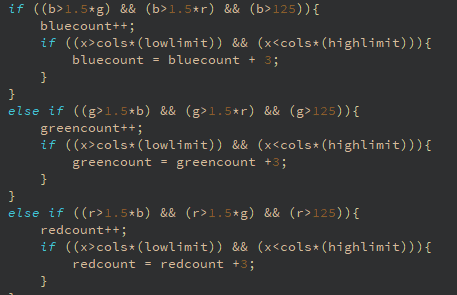
\includegraphics[width=2.5in]{t1}
%\caption{Pixel testing code}
%\label{fig_t1code}
%\end{figure}

\subsection{Limitations}

%\begin{figure}[h!]
%\centering
%\begin{subfigure}{0.225\textwidth}
%    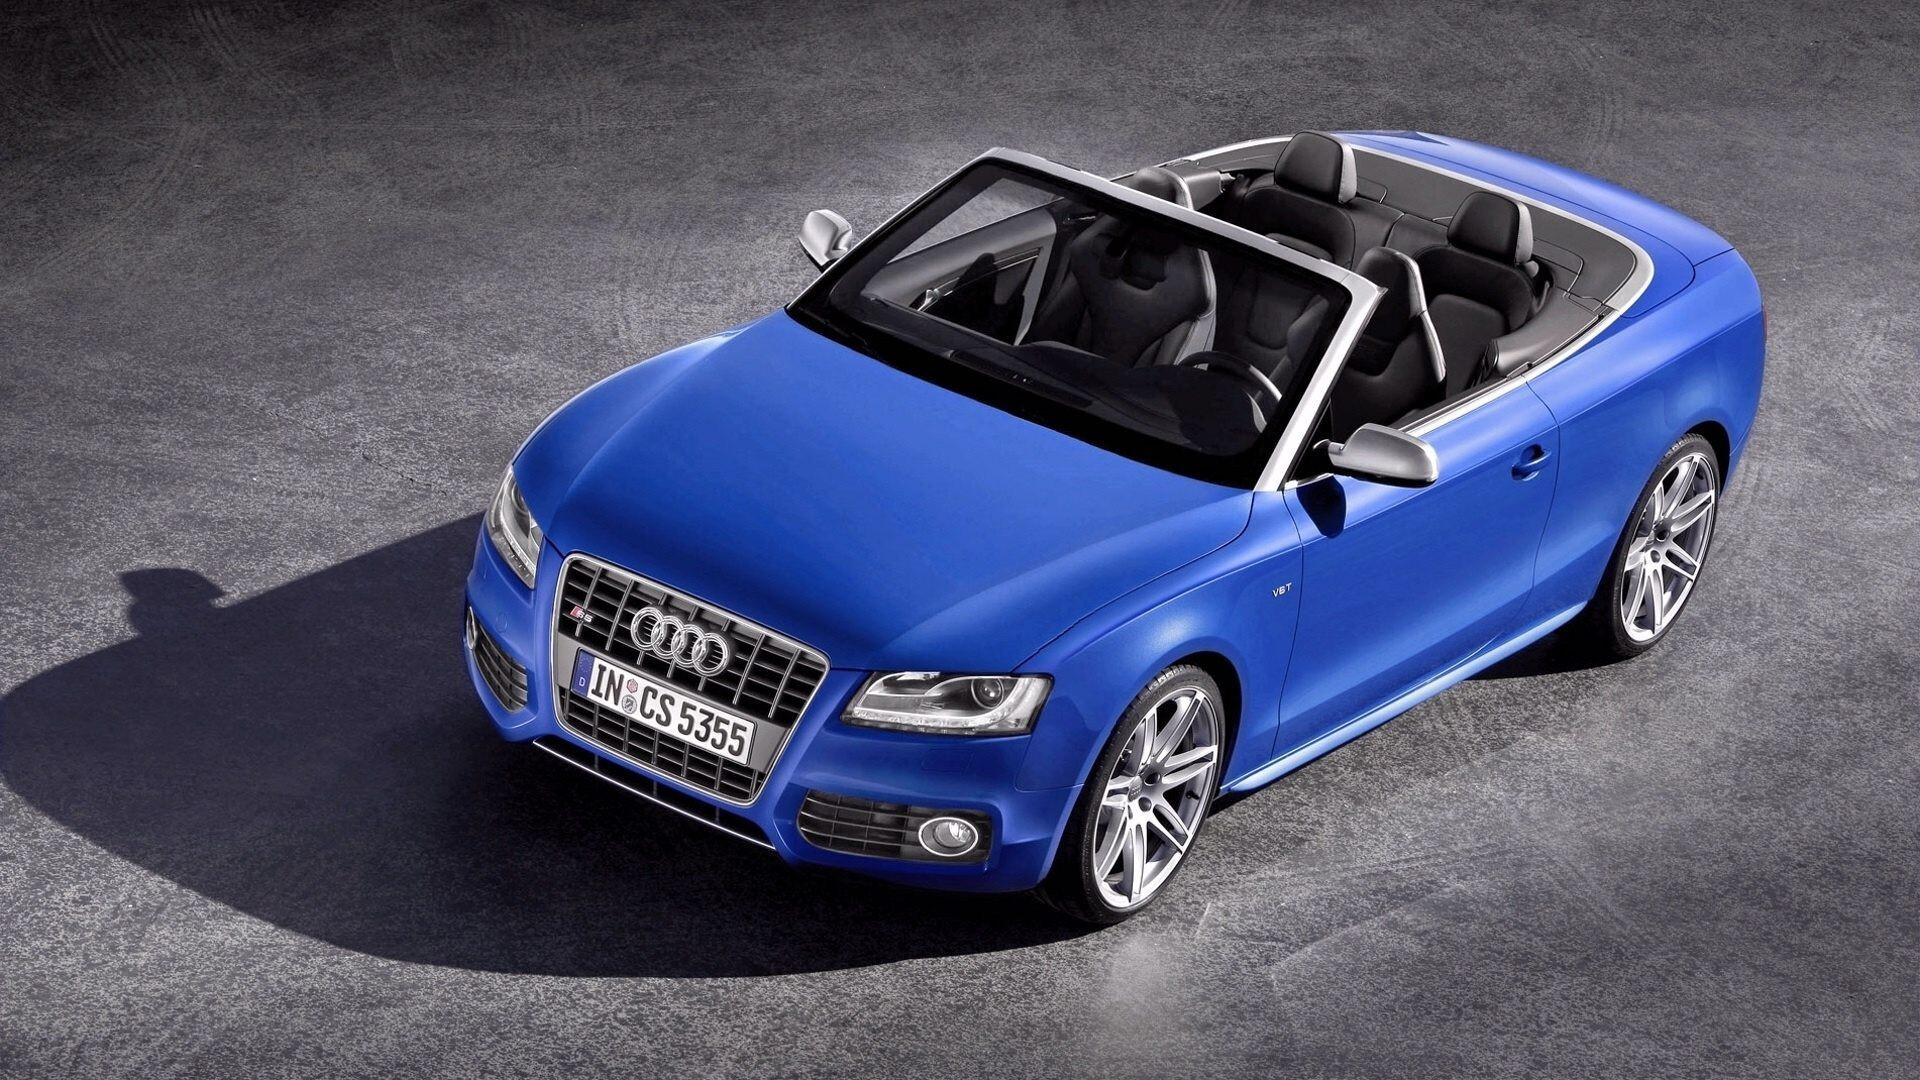
\includegraphics[width=\textwidth]{6}
%    \caption{Image 6 (Green)}
%    \label{fig:first}
%\end{subfigure}
%\hfill
%\begin{subfigure}{0.225\textwidth}
%    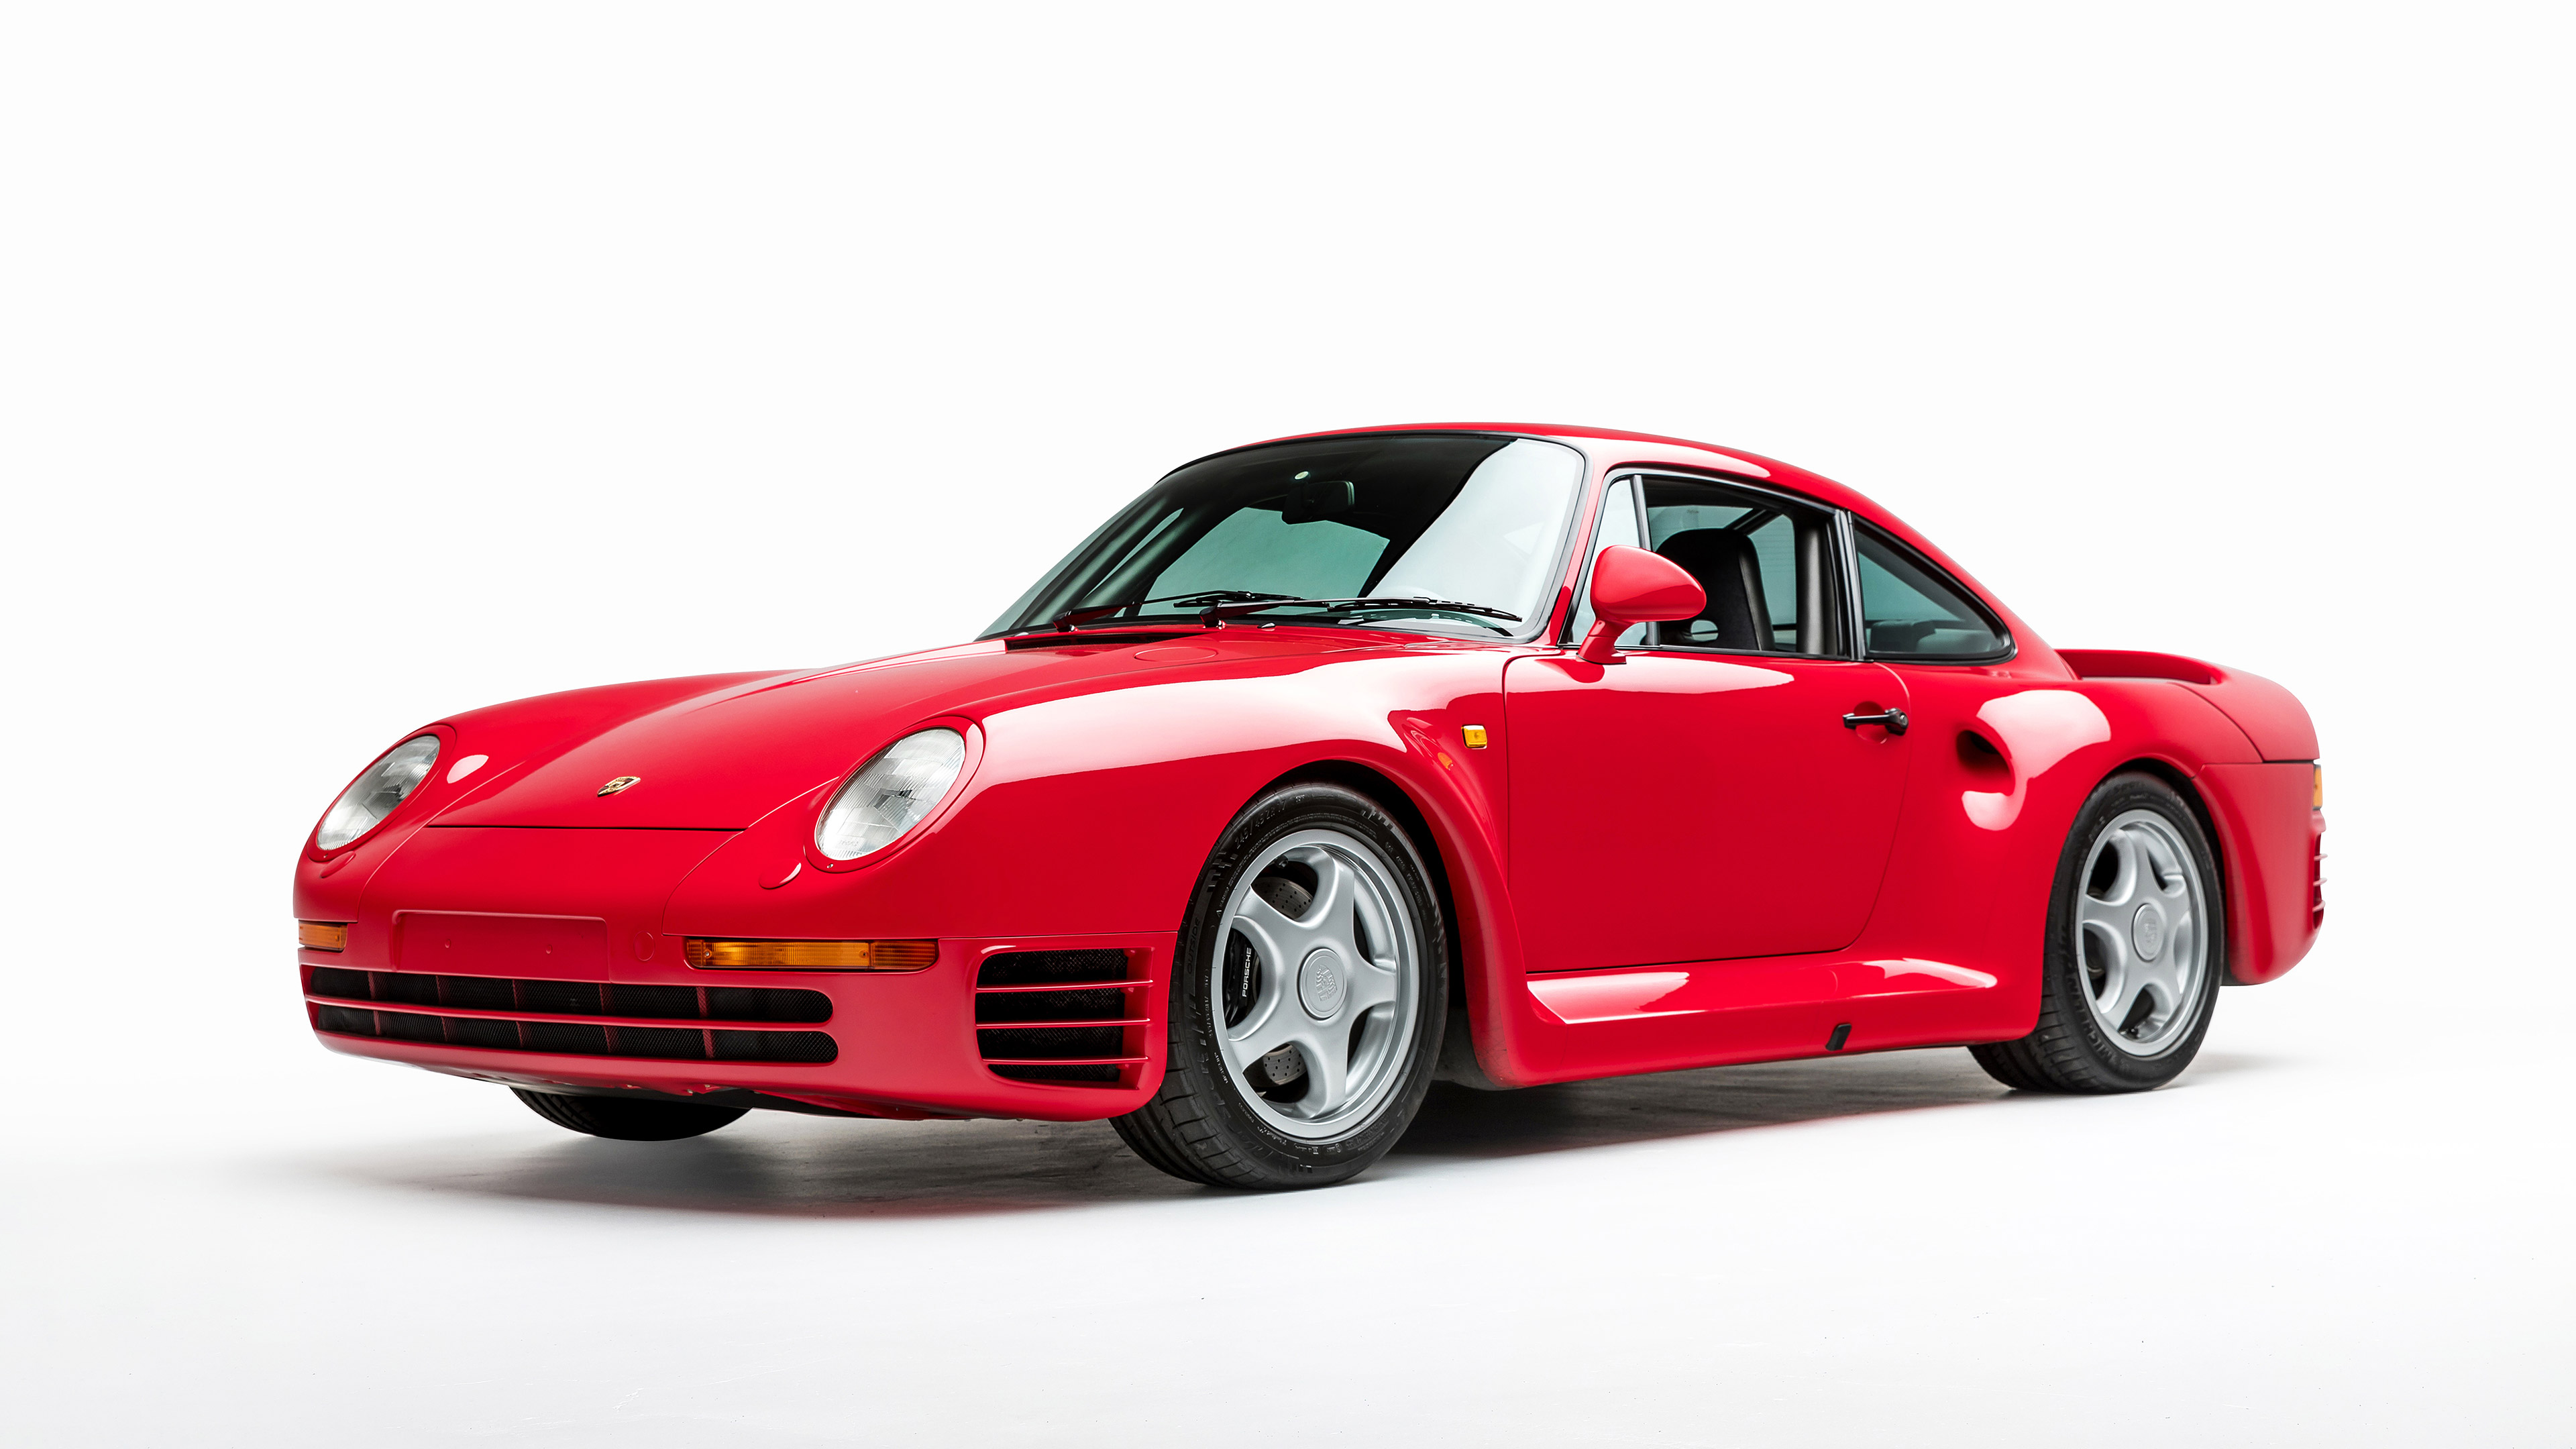
\includegraphics[width=\textwidth]{25}
%    \caption{Image 25 (Green)}
%    \label{fig:second}
%\end{subfigure}
%
%\begin{subfigure}{0.225\textwidth}
%    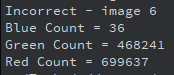
\includegraphics[width=\textwidth]{6_stats}
%    \caption{Image 6 pixel count}
%    \label{fig:third}
%\end{subfigure}
%\hfill
%\begin{subfigure}{0.225\textwidth}
%    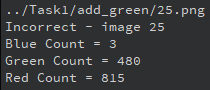
\includegraphics[width=\textwidth]{25_stats}
%    \caption{Image 25 pixel count}
%    \label{fig:fourth}
%\end{subfigure}
%
%\caption{Failed recognition images and stats}
%\label{fig:fails}
%\end{figure}

\subsection{Further Improvements} \label{sec:further1}
 
\subsection{Conclusion}

\section{Task 2 - Object Tracking}
\textit{For accompanying large figures, see appendix \ref{app:T5}}

\textit{For the video demo, click \href{https://youtu.be/kW5fbNTTovo}{HERE}}

The second task involves tracking a pendulum and using the observed displacement to calculate the pendulum's angular deviation from its vertical rest position.
\subsection{Introduction}

\subsection{Solution}\label{2_solution}

\begin{equation}
angle = x*(180/\pi )
\end{equation}


\subsection{Limitations}\label{sec:t2_lim}

\subsection{Further Improvements}

\subsection{Conclusion}

\begin{table}[]
\caption{Error values of different components.}
\label{tab:t3error}
\begin{tabular}{|l|l|}
\hline
\textbf{Component} & \textbf{NMSD Error} \\ \hline
U4                 & 0.000642183         \\ \hline
C70                & 0.000428351         \\ \hline
U2                 & 0.000984659         \\ \hline
L2                 & 0.000689957         \\ \hline
Q1                 & 0.000671107         \\ \hline
C97                & 0.000465317         \\ \hline
C87                & 0.000600116         \\ \hline
U1                 & 0.00133448          \\ \hline
U13 (Missing)      & 0.0435289           \\ \hline
U13 (Present)      & 1.52745e-07         \\ \hline
L8                 & 0.00050902          \\ \hline
\end{tabular}
\end{table}


% An example of a floating figure using the graphicx package.
% Note that \label must occur AFTER (or within) \caption.
% For figures, \caption should occur after the \includegraphics.
% Note that IEEEtran v1.7 and later has special internal code that
% is designed to preserve the operation of \label within \caption
% even when the captionsoff option is in effect. However, because
% of issues like this, it may be the safest practice to put all your
% \label just after \caption rather than within \caption{}.
%
% Reminder: the "draftcls" or "draftclsnofoot", not "draft", class
% option should be used if it is desired that the figures are to be
% displayed while in draft mode.
%
%\begin{figure}[H]
%\centering
%\includegraphics[width=2.5in]{myfigure}
% where an .eps filename suffix will be assumed under latex, 
% and a .pdf suffix will be assumed for pdflatex; or what has been declared
% via \DeclareGraphicsExtensions.
%\caption{Simulation Results}
%\label{fig_sim}
%\end{figure}

% Note that IEEE typically puts floats only at the top, even when this
% results in a large percentage of a column being occupied by floats.


% An example of a double column floating figure using two subfigures.
% (The subfig.sty package must be loaded for this to work.)
% The subfigure \label commands are set within each subfloat command, the
% \label for the overall figure must come after \caption.
% \hfil must be used as a separator to get equal spacing.
% The subfigure.sty package works much the same way, except \subfigure is
% used instead of \subfloat.
%
%\begin{figure*}[!t]
%\centerline{\subfloat[Case I]\includegraphics[width=2.5in]{subfigcase1}%
%\label{fig_first_case}}
%\hfil
%\subfloat[Case II]{\includegraphics[width=2.5in]{subfigcase2}%
%\label{fig_second_case}}}
%\caption{Simulation results}
%\label{fig_sim}
%\end{figure*}
%
% Note that often IEEE papers with subfigures do not employ subfigure
% captions (using the optional argument to \subfloat), but instead will
% reference/describe all of them (a), (b), etc., within the main caption.


% An example of a floating table. Note that, for IEEE style tables, the 
% \caption command should come BEFORE the table. Table text will default to
% \footnotesize as IEEE normally uses this smaller font for tables.
% The \label must come after \caption as always.
%
%\begin{table}[!t]
%% increase table row spacing, adjust to taste
%\renewcommand{\arraystretch}{1.3}
% if using array.sty, it might be a good idea to tweak the value of
% \extrarowheight as needed to properly center the text within the cells
%\caption{An Example of a Table}
%\label{table_example}
%\centering
%% Some packages, such as MDW tools, offer better commands for making tables
%% than the plain LaTeX2e tabular which is used here.
%\begin{tabular}{|c||c|}
%\hline
%One & Two\\
%\hline
%Three & Four\\
%\hline
%\end{tabular}
%\end{table}


% Note that IEEE does not put floats in the very first column - or typically
% anywhere on the first page for that matter. Also, in-text middle ("here")
% positioning is not used. Most IEEE journals/conferences use top floats
% exclusively. Note that, LaTeX2e, unlike IEEE journals/conferences, places
% footnotes above bottom floats. This can be corrected via the \fnbelowfloat
% command of the stfloats package.


\newpage
\appendix

\printbibliography


\onecolumn
\subsection{Github Repository}

For the full code, please see the linked github repository \href{https://github.com/jjpendlebury/AINT308-Coursework}{HERE}.
\subsection{Task 4 Figures}\label{app:T4}


\subsection{Task 5 Figures}\label{app:T5}

\subsection{Code Printouts}
The following pages contain complete printouts of the code used to implement the solutions outlined above, for reference.
%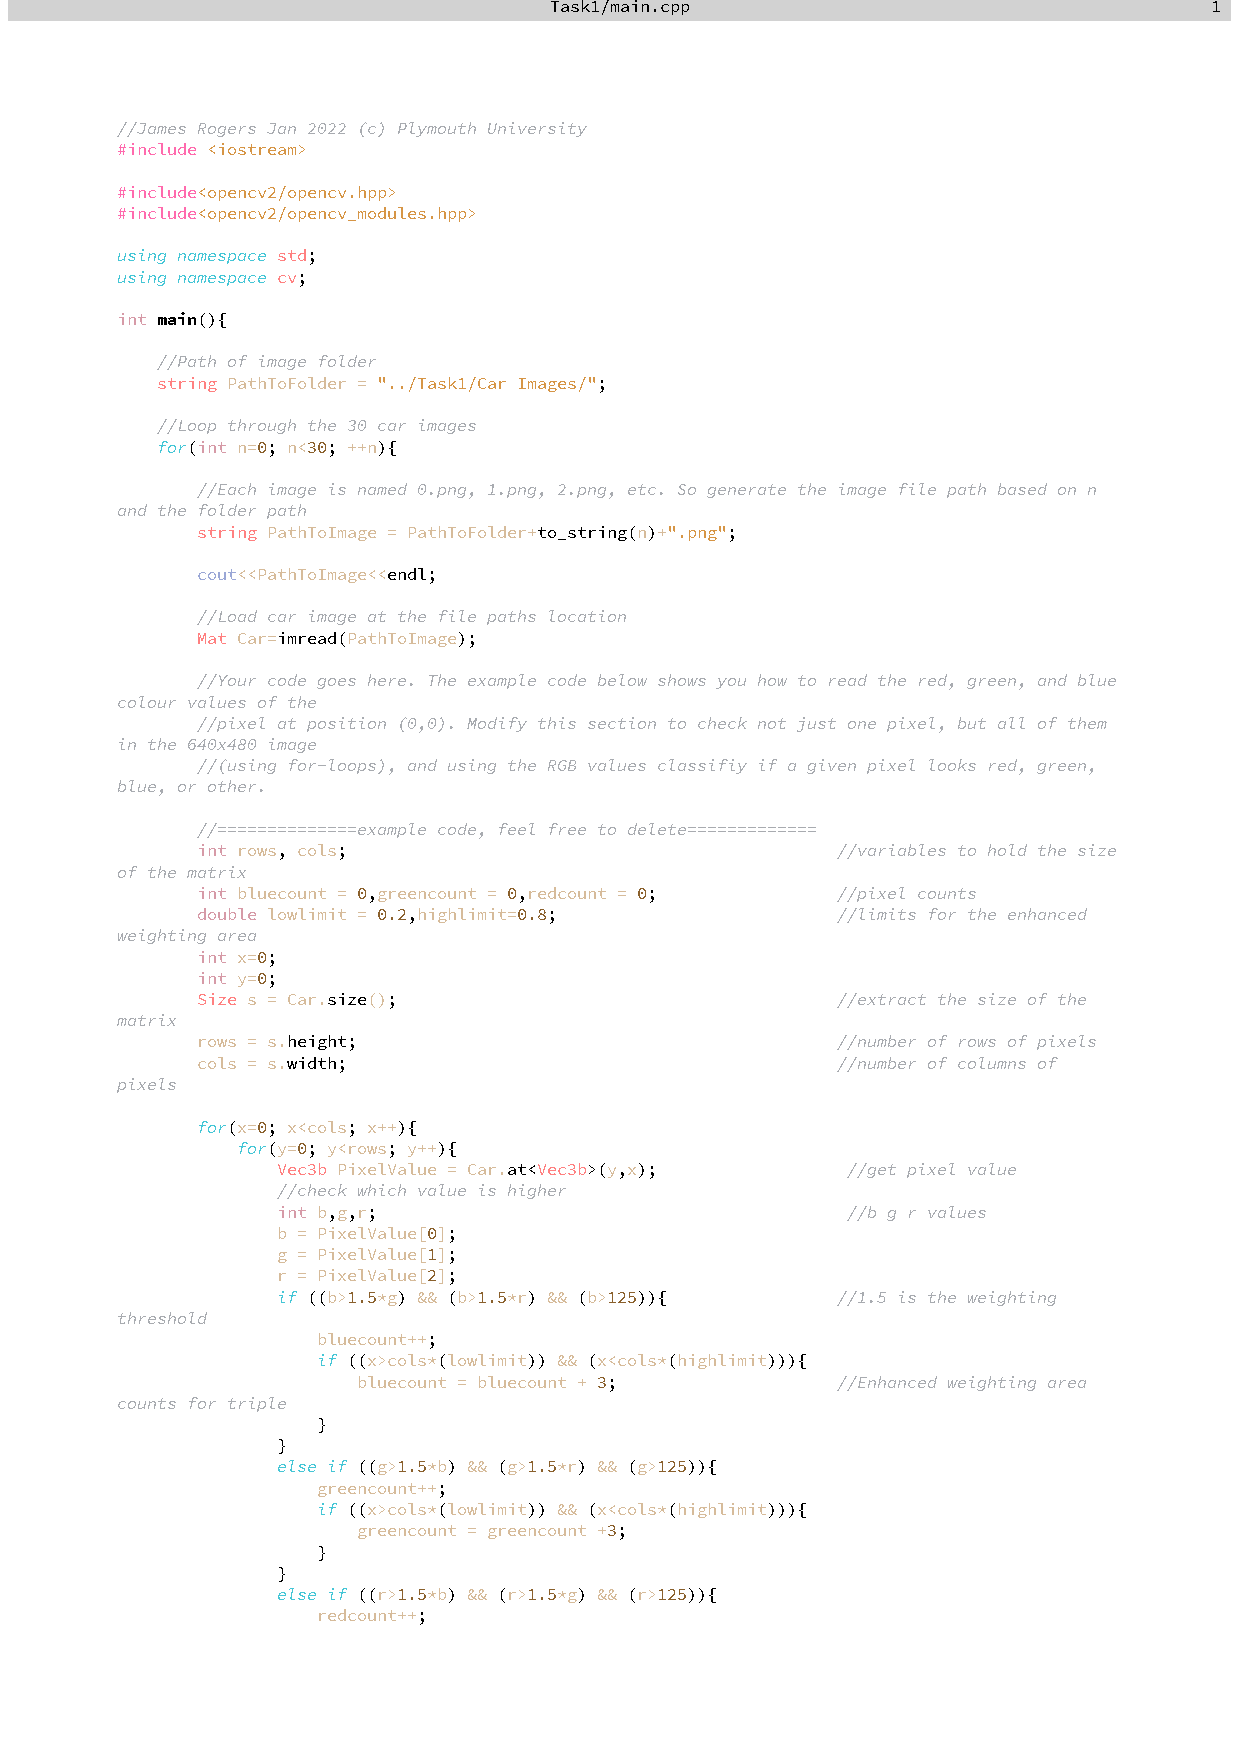
\includepdf[pages=-,offset=0 -50]{task1_code.pdf}
%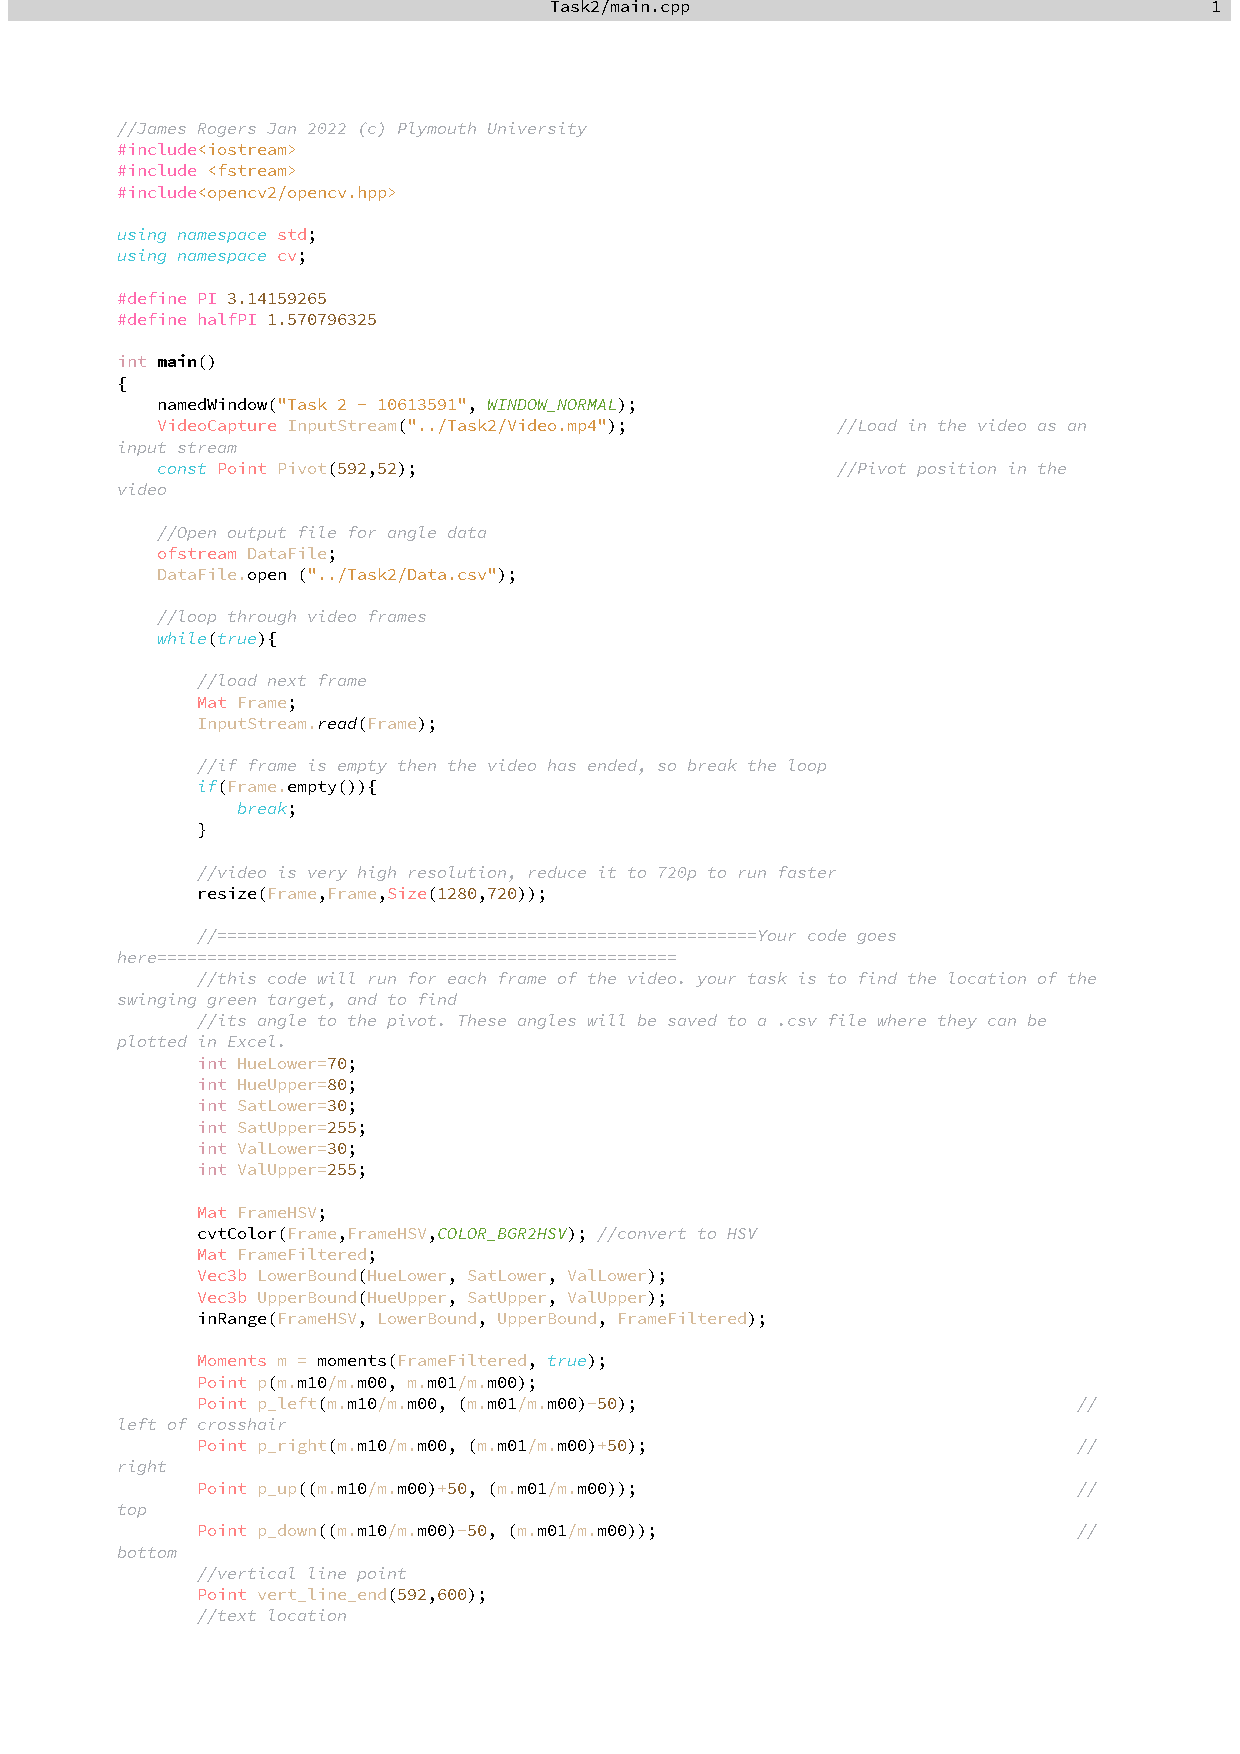
\includepdf[pages=-,offset=0 -50]{task2_code.pdf}
%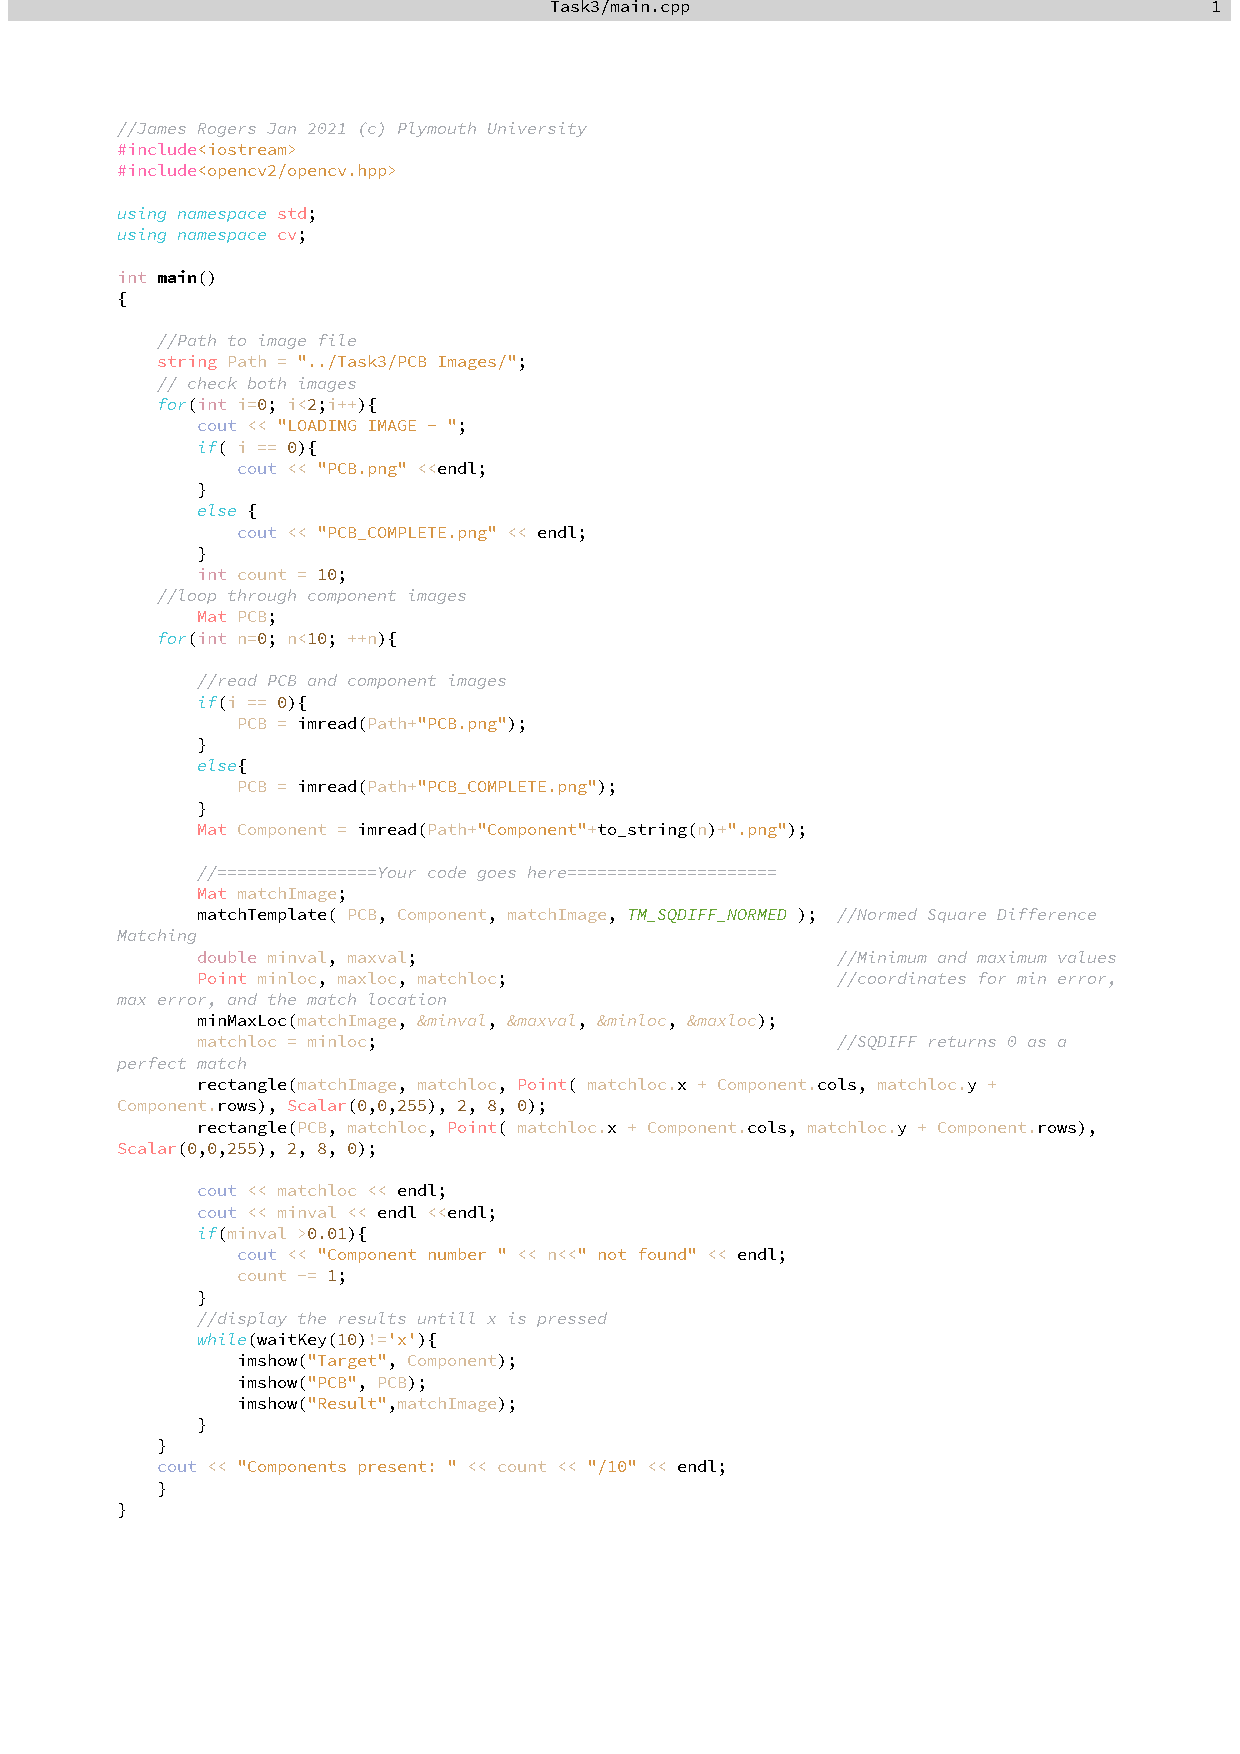
\includepdf[pages=-,offset=0 -50]{task3_code.pdf}
% that's all folks
\end{document}